\subsection{Protocols}

Protocols are user-level applications for consensus, defined as arbitrary time-dependent functions acting on the current state of the broadcast channel,
\begin{align}
	\textsc{Protocol}(\mathcal{B}(t=0),\star)\to \star,
\end{align}
where time is relative to the present. The state of the broadcast channel a time $t$ contains all previous messages broadcasts,
where,
\begin{align}
	\mathcal{B}(t=0) = \bigcup_{x\in \mathcal{B}(t\leq 0)} x.
\end{align}

The state of the broadcast channel is in general subjective as individual users may have imperfect knowledge of $\mathcal{B}$ as a result of information loss. The subjective state of the broadcast channel for user $i$ is,
\begin{align}
	\mathcal{B}_i \subseteq \mathcal{B}.
\end{align}
Consequently, \textsc{Protocol} outputs are also subjective and may differ in general,
\begin{align}
	\textsc{Protocol}_i(\mathcal{B}_i,\star) \neq \textsc{Protocol}(\mathcal{B},\star)
\end{align}

* Interfaces

\subsection{Distributed filesystems}

* Object storage counters. Promise in units of bit-seconds.

* Owner and anonymous ownership models.

* Quasi-persistent storage model.

* Dynamically load-balanced under randomisation.

* Encoding density vs readout ability within islands of fractured network.

\subsubsection{Object stores}

\begin{figure}[!htp]
	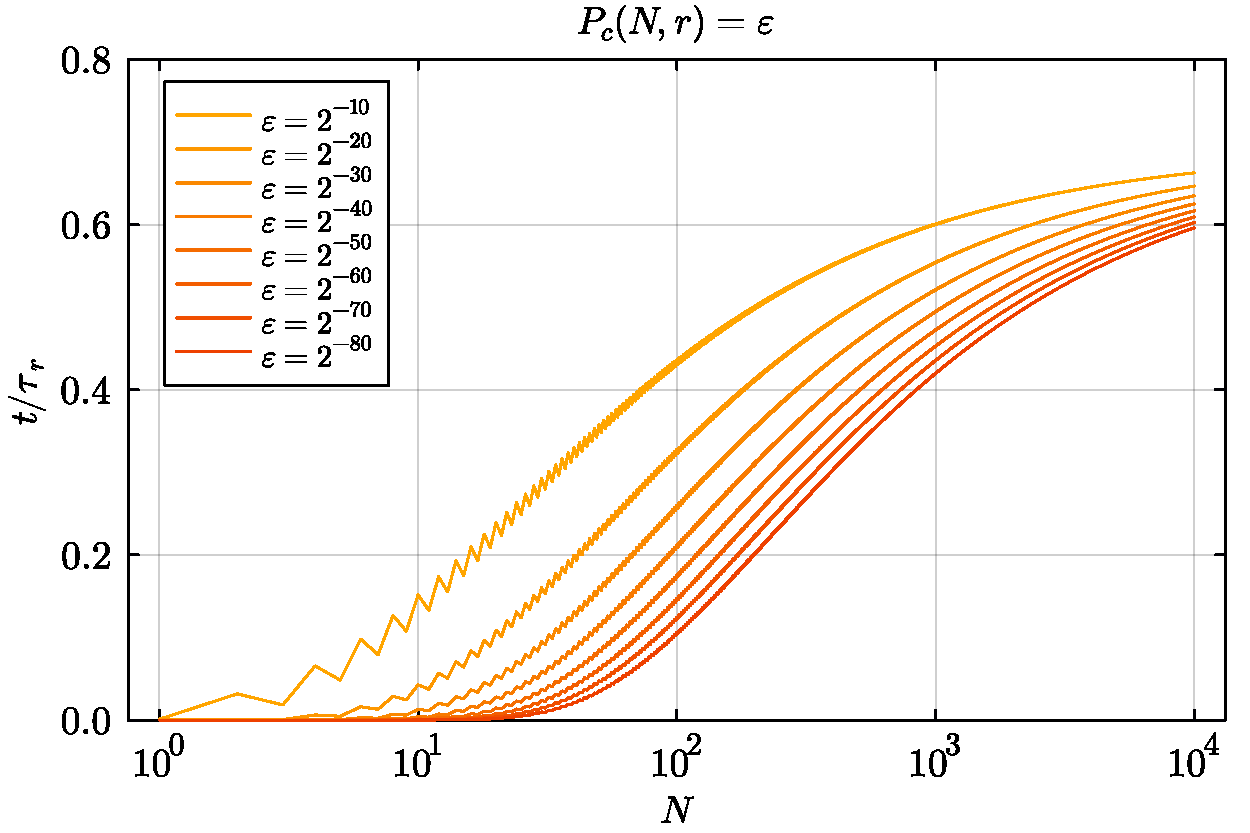
\includegraphics[width=\columnwidth]{figs/DObS_time.pdf}\\
	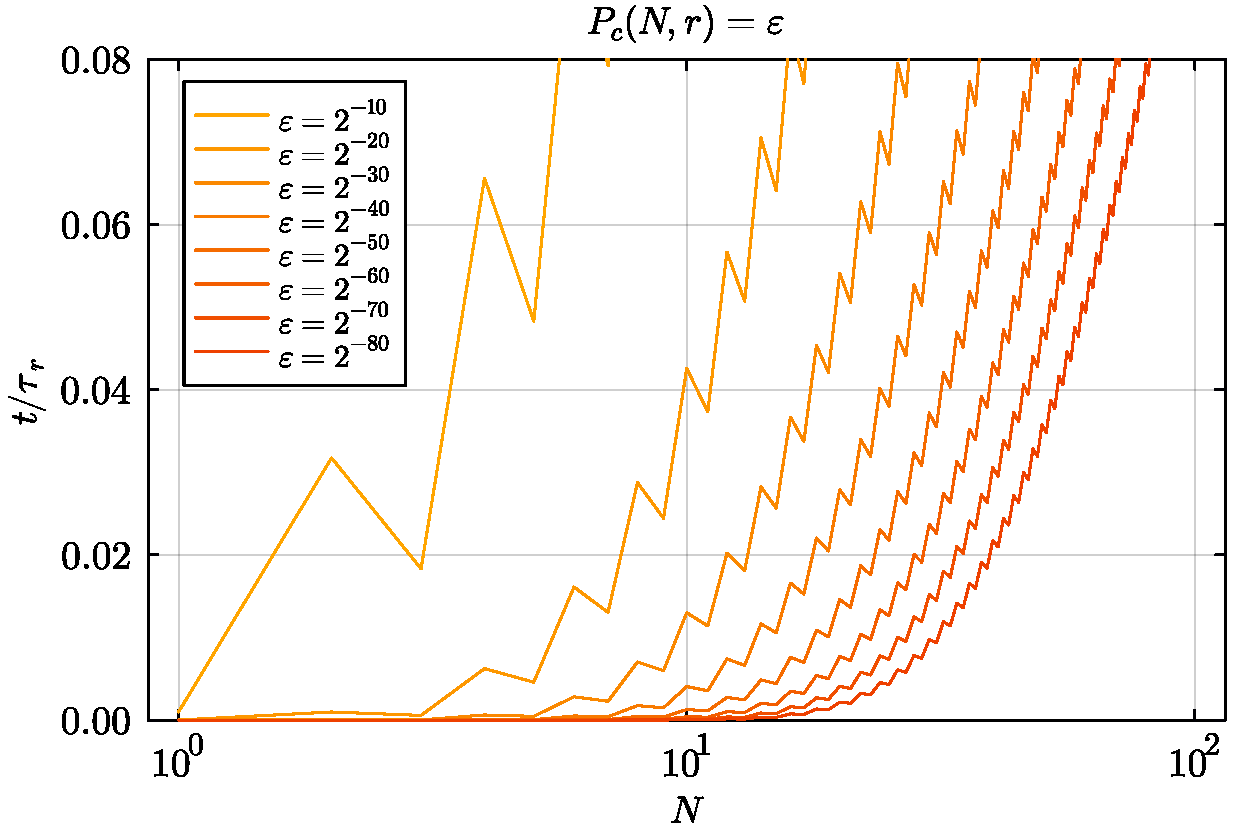
\includegraphics[width=\columnwidth]{figs/DObS_time_zoom.pdf}
	\caption{\textbf{Security tradeoffs between consensus set size and object storage lifetime.} Using $r(0)=0$. Corresponds to Fig.~\ref{fig:P_M}.} \label{fig:DObS_time}
\end{figure}

\begin{figure}[!htp]
	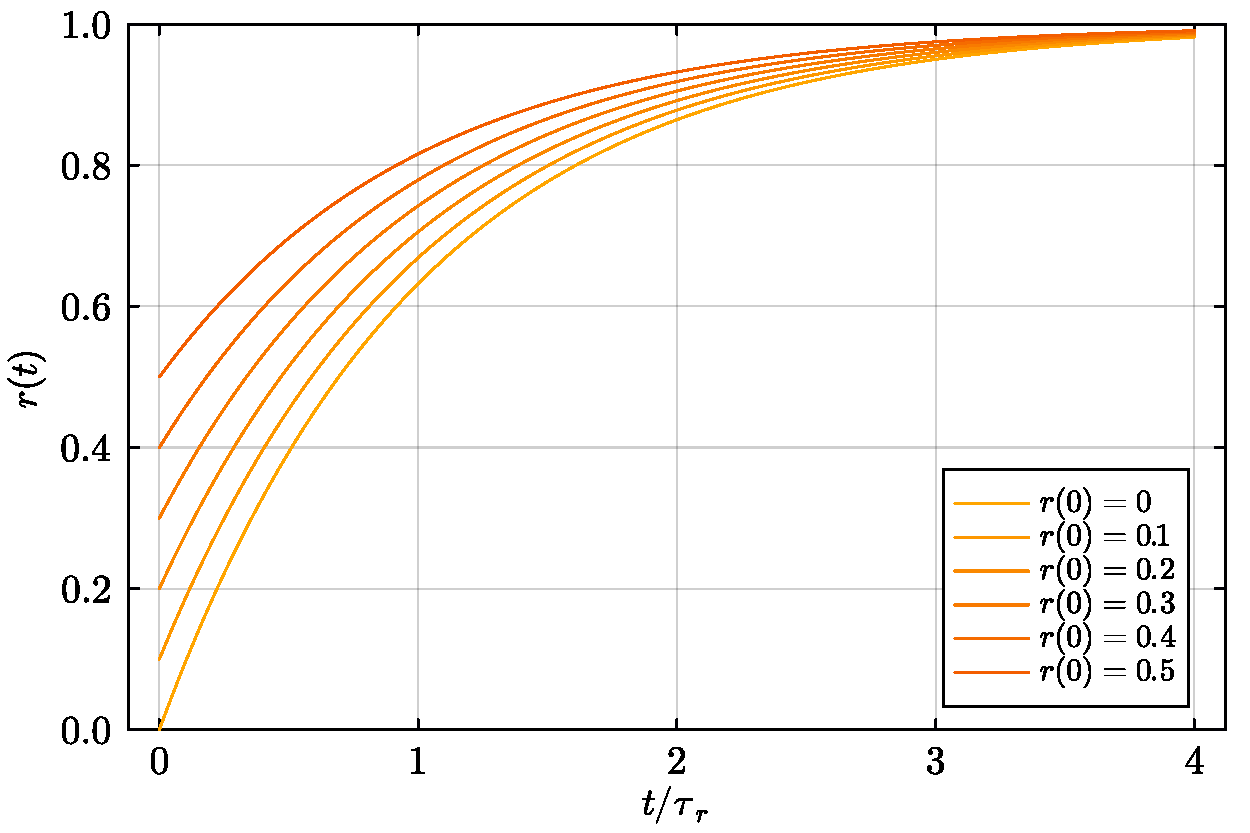
\includegraphics[width=\columnwidth]{figs/DObS_r_time.pdf}\\
	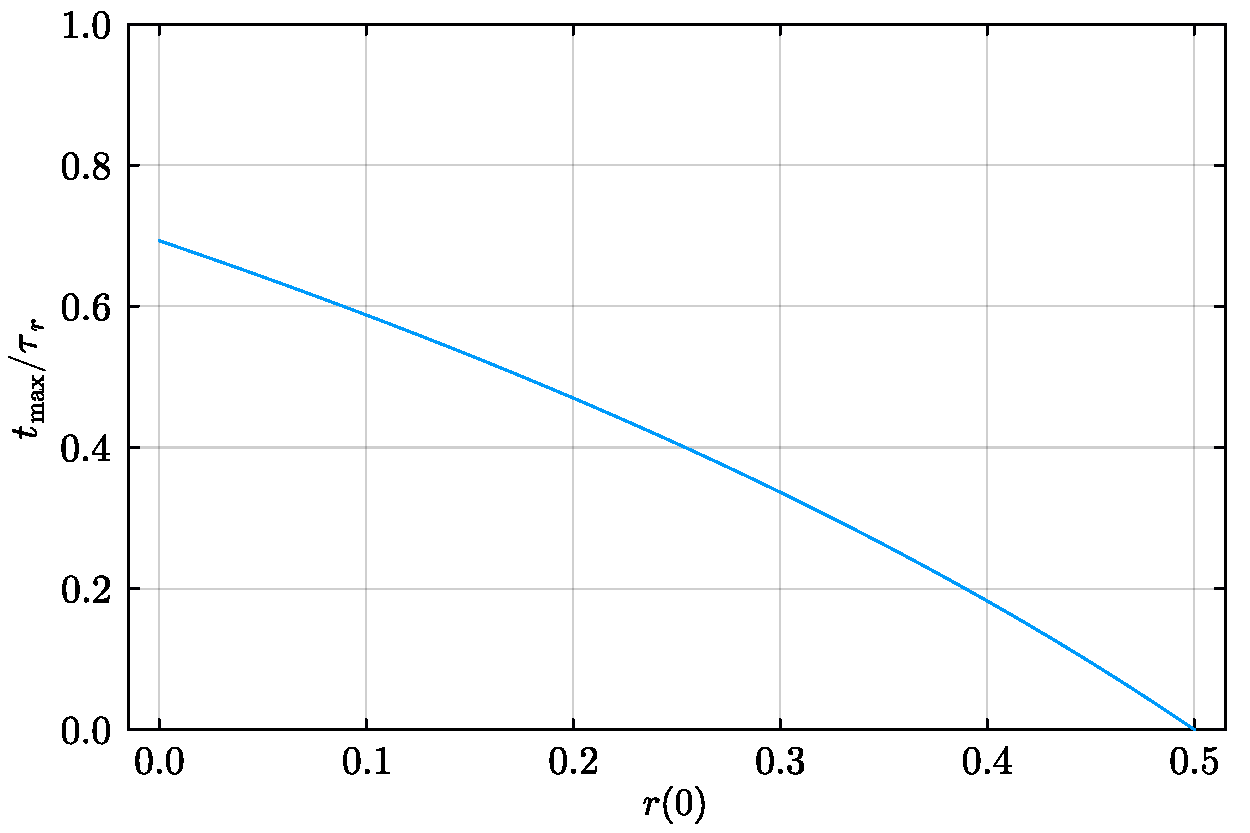
\includegraphics[width=\columnwidth]{figs/DObS_max_time.pdf}
	\caption{\textbf{Maximum object lifetime.} For $N_C\to\infty$.} \label{fig:DObS_max_time}
\end{figure}

* Object or blob storage.

* Lifetime/consensus set size tradeoff for $\varepsilon$-security. Consider exponential decay model, interpreted as ...,
\begin{align}
	r(t) = 1-[1 - r(0)]\, e^{-t/\tau_r}.
\end{align}

* Asymptotic for $r(t)=1/2$ as $N_C\to\infty$,
\begin{align}
	t_\mathrm{max}=\tau_r \log[2-2r(0)]
\end{align}

* See Fig.~\ref{fig:DObS_time}

* See Fig.~\ref{fig:DObS_max_time}

* All nodes locally record the hashes of all segments. Consensus is formed upon agreement of the hash-list. Converts malicious nodes to segment erasure.

Consider an object storage model, a structurally flat persistent storage model in which arbitrary data objects are the primitive storage unit, residing in an object store (ObS) \cite{ObjectStore}.

Object stores supports the CRUD query primitives to \textsc{Create}, \textsc{Read}, \textsc{Update} and \textsc{Delete} objects (or \textsc{Insert}, \textsc{Select}, \textsc{Update} and \textsc{Delete} in SQL database terminology).

Scalable distributed objects stores (DObS) must support \emph{concurrency control}, the ability to safely execute multiple object queries simultaneously without causing race conditions, yielding undefined outcomes or data corruption.

Concurrency control requires serialisation of conflicting operations on common data, often implemented using mutual exclusion (mutex) synchronisation primitives, analogous to ensuring thread-safety in asynchronous programming environments. The \emph{actor model} for concurrency mitigates race conditions by assigning operations on a common object to a single execution thread -- the \emph{actor} -- which executes them synchronously \cite{ActorModel}.

DCN object stores assign consensus sets as actors on object queries, where consensus set $\mathcal{C}(\texttt{obj}_x)$ is assigned as the actor for object $\texttt{obj}_x$. Nodes in $\mathcal{C}(\texttt{obj}_x)$ are exclusively responsible for storing and querying $\texttt{obj}_x$.

Bids may now encapsulate object queries, where \textsc{Create} queries are executed by newly-assigned consensus sets, while \textsc{Read} and \textsc{Delete} queries are executed by the consensus sets the respective object was initially assigned to.

* Predicates. Nodes independently evaluate queries. Queries operating on objects for which a node is an actor are dispatched to consensus tasks, which are inherently thread-safe and may be executed asynchronously.

* DObS write: All nodes calculate list of all segment hashes.

Let $d^{(enc)}_{i,j}$ be information symbol $j$ held by node $i$ during encoding, and,
\begin{align}
	h_{i,j}=\textsc{Hash}(d_{i,j}^{(enc)}),
\end{align}
the respective reported hash. Consensus is formed upon the hash list $h^{(con)}$.

DObS read: Consensus formed on which segments are correctly recovered:
\begin{align}
	e_{i,j} = [\textsc{Hash}(d_{i,j}^\text{(dec)}) = h_j^\text{(con)}],
\end{align}
where $[\cdot]$ denotes the Iverson bracket. Outcome is consensus-agreed hash list upon encoding, $h^\text{(enc)}$.

* What about update?

* Since consensus outcomes either succeed or fail queries are inherently atomic.

* Since consensus inherently timestamps operations the object store is inherently \emph{versioned}.

\subsubsection{Distributed erasure codes}

Object stores must afford high storage reliability and integrity. In a distributed environment with variable node participation and and non-zero node storage failure this requires redundancy to maintain high likelihood of object retrieval.

Most simply, this may be implemented using \emph{mirroring} whereby multiple copies of data are stored independently as backups should some become unavailable, the approach used in RAID (type 1) storage arrays. More generally, data redundancy may be implemented using error correcting codes (ECCs).

There are two primary error models ECCs may be applied to:
\begin{itemize}
	\item Bit errors: Bits are randomly subject to bit-flips. In the absence of error detection these are \emph{unlocated errors}, meaning it is not known where they occurred.
	\item Erasure errors: Bits are randomly lost. These will be treated as \emph{located errors} where their location is known.
\end{itemize}

The error-correcting properties of block ECCs are characterised by,
\begin{align}
	[n,k,d],
\end{align}
for a code encoding $k$ information bits into length $n$ codewords with code distance $d$ (the minimum Hamming distance between any two codewords). The code's rate is given by,
\begin{align}
	r = \frac{k}{n}.
\end{align}

In general, the information provided by known error locations enables erasure codes to exhibit higher error tolerance than bit-error codes. Specifically, an ECC can correct twice as many erasures ($E$) as errors ($S$), following the tradeoff inequality,
\begin{align}
	2E+S \leq d.
\end{align}

Fountain codes \cite{Fountain, RepFountainCodes, MackayFountain} are a class of ECCs exhibiting the \emph{fountain properties}:
\begin{itemize}
	\item Any subset of $k$ encoded symbols is sufficient to decode the source symbols with high probability. Fountain codes are \emph{rateless} since the number of erasures may be arbitrary so long as the required number of codeword symbols are received.
	\item Encoding and decoding operations exhibit linear time-complexity, $O(k)$.
\end{itemize}

Fountain code codewords are constructed by bitwise XORing random subsets of information symbols according to the code's Tanner graph (Fig.~\ref{fig:tanner_graph}), with degree sequence sampled from a probability distribution $P_D(x)$.

\begin{figure}[!htb]
	\begin{tikzpicture}[]
    \def\UVsep{2.8}

    \tikzset{oplus node/.style={inner sep=0pt, minimum size=1em, label=center:{\scalebox{1.5}[1.5]{$\oplus$}}}}
    \tikzset{circ node/.style={inner sep=0pt, minimum size=1em, label=center:{\scalebox{1.5}[1.5]{$\Circle$}}}}

    \node[circ node] (a1) at (0,-1) {};
    \node[circ node] (a2) at (0,-2) {};
    \node[circ node] (a3) at (0,-3) {};
    \node[circ node] (a4) at (0,-4) {};
    \node[draw=none] (a5) at (0,-5) {$\vdots$};
    \node[circ node] (a6) at (0,-6) {};
    
    \node[oplus node] (b1) at (\UVsep,-1) {};
    \node[oplus node] (b2) at (\UVsep,-2) {};
    \node[oplus node] (b3) at (\UVsep,-3) {};
    \node[oplus node] (b4) at (\UVsep,-4) {};
    \node[oplus node] (b5) at (\UVsep,-5) {};
    \node[draw=none] (b6) at (\UVsep,-6) {$\vdots$};
    \node[oplus node] (b7) at (\UVsep,-7) {};

    \node[draw=none, left=0em of a1] (labela1) {$x_1$};
    \node[draw=none, left=0em of a2] (labela2) {$x_2$};
    \node[draw=none, left=0em of a3] (labela3) {$x_3$};
    \node[draw=none, left=0em of a4] (labela4) {$x_4$};
    \node[draw=none, left=0em of a6] (labelak) {$x_k$};

    \node[draw=none, right=0em of b1] (labelb1) {$c_1$};
    \node[draw=none, right=0em of b2] (labelb2) {$c_2$};
    \node[draw=none, right=0em of b3] (labelb3) {$c_3$};
    \node[draw=none, right=0em of b4] (labelb4) {$c_4$};
    \node[draw=none, right=0em of b5] (labelb4) {$c_5$};
    \node[draw=none, right=0em of b7] (labelbn) {$c_n$};

    \foreach \i in {1,...,6} {
            \ifnum\i=5
            \else
                \foreach \j in {1,...,7} {
                    \ifnum\j=6
                        \else
                        \draw[graphNonEdgeStyle, line width=0.5] ($(a\i.east) + (0.01,0)$) -- ($(b\j.west) + (-0.01,0)$);
                    \fi
                }
            \fi
        }

    \draw[graphEdgeStyle, line width=0.5] ($(a1.east) + (0.01,0)$) -- ($(b1.west) + (-0.01,0)$);
    \draw[graphEdgeStyle, line width=0.5] ($(a1.east) + (0.01,0)$) -- ($(b3.west) + (-0.01,0)$);
    \draw[graphEdgeStyle, line width=0.5] ($(a1.east) + (0.01,0)$) -- ($(b7.west) + (-0.01,0)$);

    \draw[graphEdgeStyle, line width=0.5] ($(a2.east) + (0.01,0)$) -- ($(b2.west) + (-0.01,0)$);
    \draw[graphEdgeStyle, line width=0.5] ($(a2.east) + (0.01,0)$) -- ($(b3.west) + (-0.01,0)$);
    \draw[graphEdgeStyle, line width=0.5] ($(a2.east) + (0.01,0)$) -- ($(b5.west) + (-0.01,0)$);

    \draw[graphEdgeStyle, line width=0.5] ($(a3.east) + (0.01,0)$) -- ($(b3.west) + (-0.01,0)$);
    \draw[graphEdgeStyle, line width=0.5] ($(a3.east) + (0.01,0)$) -- ($(b5.west) + (-0.01,0)$);

    \draw[graphEdgeStyle, line width=0.5] ($(a4.east) + (0.01,0)$) -- ($(b2.west) + (-0.01,0)$);
    \draw[graphEdgeStyle, line width=0.5] ($(a4.east) + (0.01,0)$) -- ($(b4.west) + (-0.01,0)$);
    
    \draw[graphEdgeStyle, line width=0.5] ($(a6.east) + (0.01,0)$) -- ($(b4.west) + (-0.01,0)$);
    \draw[graphEdgeStyle, line width=0.5] ($(a6.east) + (0.01,0)$) -- ($(b5.west) + (-0.01,0)$);
    \draw[graphEdgeStyle, line width=0.5] ($(a6.east) + (0.01,0)$) -- ($(b7.west) + (-0.01,0)$);
    
    \node[draw=none] at ($(a1.east)!0.5!(b1.west) + (0,0.25)$) {$P_D(x)$};
\end{tikzpicture}
	\caption{\textbf{Tanner graph for fountain codes.} The Tanner graph captures which information symbols ($x_i$) combine under bitwise XOR to produce the respective codeword symbols ($c_j$) according to edge existence. The degree sequence $d(x)$ is randomly sampled from a probability distribution $P_D(x)$ specific to the code. For Fountain codes, receiving any $k+o$ codeword symbols guarantees decoding with high probability.}\label{fig:tanner_graph}
\end{figure}

Luby transform (LT) codes \cite{LTCodes} were the first practical realisation of fountain codes where $k$ information symbols are recoverable from any set of,
\begin{align}
	k+o = k+O(\sqrt{k} \log^2(k/\delta)),
\end{align}
codeword symbols with success probability,
\begin{align}
	P_\mathrm{rec}=1-\delta,
\end{align}
using a decoding algorithm with,
\begin{align}
	O(k \log(k/\delta)),
\end{align}
time-complexity, where $o$ is the code's overhead.

For LT codes an optimal degree sequence distribution is the Ideal Soliton distribution,
\begin{align}
	P_D(x) = \begin{cases}
 		\frac{1}{k}, &x=1,\\
 		\frac{1}{x(x-1)}, &2\leq x\leq k.
	\end{cases}
\end{align}

The efficiency of LT codes may be enhanced using Raptor codes \cite{RaptorCodes, RaptorCodes2}, composing an LT code with a conventional block erasure pre-code such as Tornado codes \cite{TornadoCodes}.

Objects are in general sparsely encoded in a DCN-ObS since $N\gg n$, where,
\begin{align}
	r_\mathrm{enc}=\frac{k+o}{n},
\end{align}
is the encoding density. Since $n=|\mathcal{C}|$ can be treated as a constant for given security/data recoverability thresholds, encoding density scales as $r_\mathrm{enc}=O(1/N)$.

Encoding $k$ information symbols across a consensus set of size $N_C$ affords an overhead of,
\begin{align}
	o = N_C - k,
\end{align}
with respective object loss probability,
\begin{align}
	\delta = O\left(\exp\left[-\sqrt{\frac{r_f N_C-k}{\sqrt{k}}} \right]\right),
\end{align}
for node storage failure rate $r_f$ (Fig.~\ref{fig:fountain}).

\begin{figure}[!htb]
	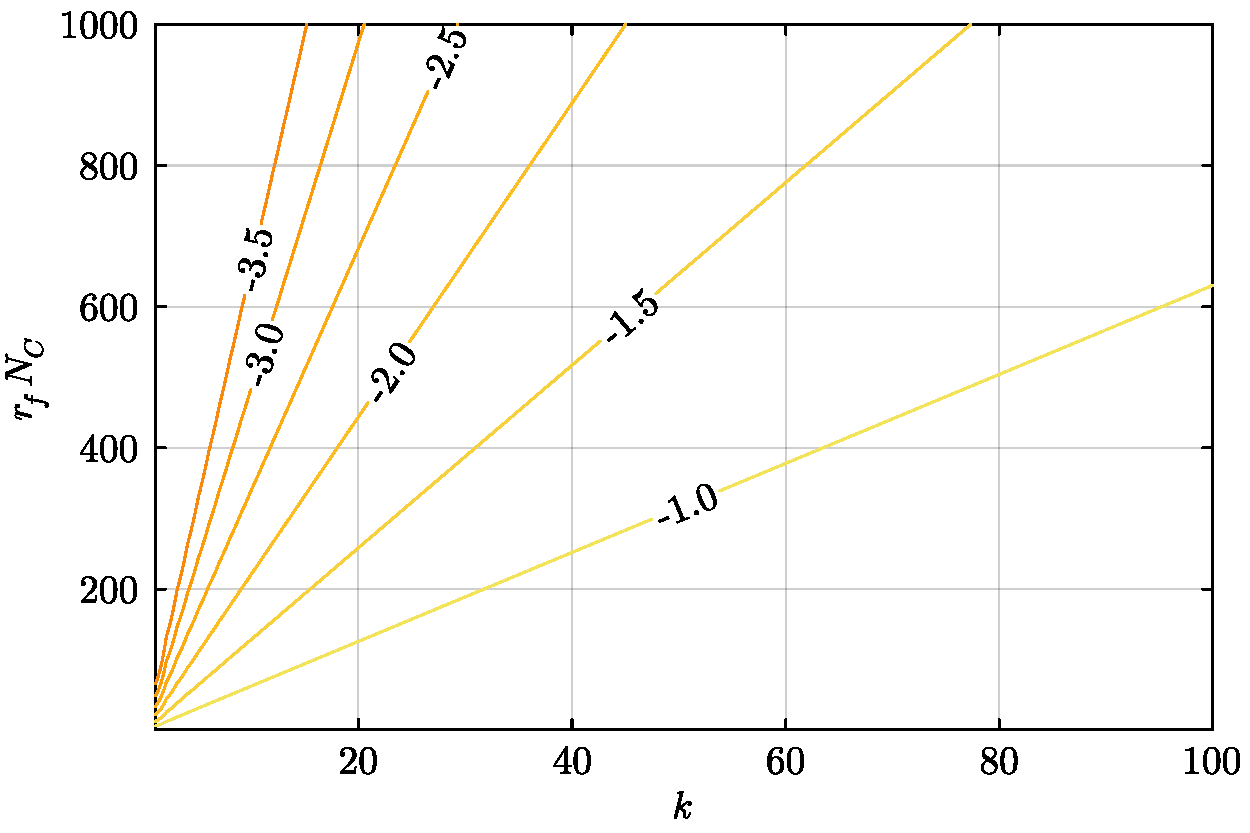
\includegraphics[width=\columnwidth]{figs/fountain.pdf}
	\caption{\textbf{Object recovery probability using a distributed fountain code.} $k$ information symbols are encoded across a consensus set of size $N_C$ with node storage failure rate $r_f$. Contours lines show $\log_\mathrm{10}(\delta)$.} \label{fig:fountain}
\end{figure}

* Treating $P_\mathrm{dec}$ as the ObS 

\begin{figure}[!htb]
	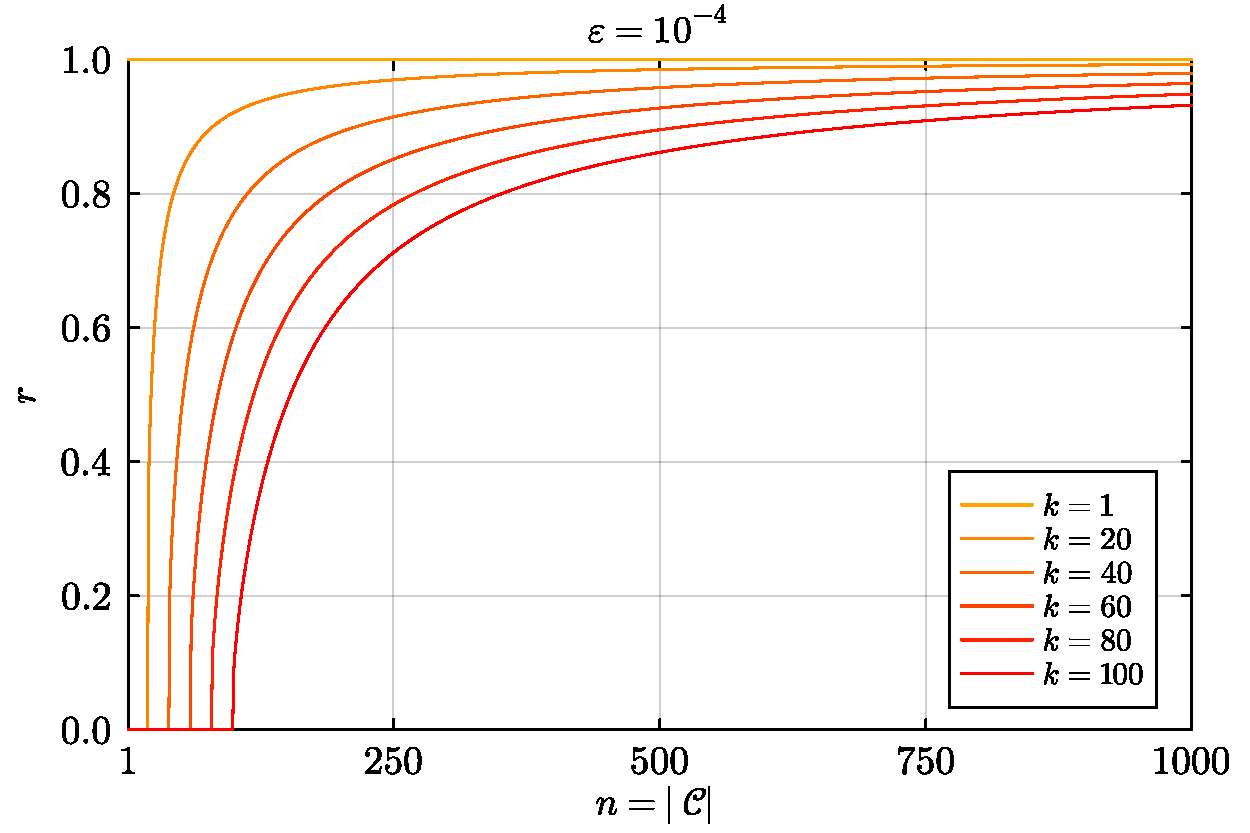
\includegraphics[width=\columnwidth]{figs/DCNFS.pdf}
	\caption{\textbf{???.}} \label{fig:DCNFS}
\end{figure}

* Fig.~\ref{fig:DCNFS}.

* To ensure consistent interpretation of the degree sequence $d(x)$ across nodes $P_D(x)$ is seeded by the network's shared random variable $\mathcal{X}_\mathcal{N}$, yielding $P_D^{(\mathcal{X}_\mathcal{N})}(x)$.

* Primitive storage operations are \textsc{Insert}, \textsc{Remove} and \textsc{Modify}.

* Sparse storage for $N\gg n$.

* Liquid cloud storage: \cite{LiquidCloudStorage}

\begin{align}
	k_\mathrm{maj} = \lfloor N/2 \rfloor + 1.
\end{align}
Hence, the likelihood of compromise is,
\begin{align}
	P_C(N,r) = I_r(\lfloor N/2 \rfloor + 1,N-\lfloor N/2 \rfloor).
\end{align}

* Could use any block erasure code.

To apply fountain codes to distributed storage we subdivide arbitrary data objects into $k$ segments forming the input symbols to the code. From the input symbols $n$ unique codewords are prepared, which are distributed and stored across $n$ nodes. So long as $k$ of the $n$ nodes are compliant the input symbols are recoverable. The likelihood of successful data recovery is analogous to Eq.~\eqref{eq:rss_probability},
\begin{align}
	P_R(n,k,r_f) & = \sum_{k'=k}^{n} \binom{n}{k'} {r_f}^{n-k'} (1-r_f)^{k'} \nonumber \\
	         & = ???%I_{r_f}(k,n-k+1),
\end{align}
where $r_f$ is the node failure rate and \mbox{$n=|\mathcal{C}|$} since objects are stored only by their respective consensus set actors.

\subsection{Distributed computational models}

\subsubsection{\textsc{MapReduce} model}

The consensus assignment problem may be interpreted more generically as randomised dynamic load allocation.

Consider the case of $|\mathcal{C}|=1$ consensus sets, the delegation of computational workloads to single randomly allocated nodes. In this context the consensus assignment algorithm facilitates dynamic load balancing across the network. Similarly, \mbox{$|\mathcal{C}|>1$} equates to dynamic allocation with $|\mathcal{C}|$-fold redundancy where consensus is formed on the outcome.

More generally, \textsc{MapReduce}-type \cite{MapReduce} computations may be delegated to consensus sets of arbitrary size, where the \textsc{Map} routine corresponds to the assignment of consensus nodes and the \textsc{Reduce} routine is evaluated by consensus.

* Distributed queries.

* Consider asymmetric bidding if preserving $r$ is not a consideration.

\subsubsection{Virtual thread pools}

* Parallel and concurrent models allow interprocess communication via observation of objects owned by other actors.

\subsubsection{Transactional model}

DCNs naturally lend themselves to a \emph{transactional model} for computation. Let \mbox{$\mathcal{S}\subseteq\mathcal{N}$} denote a subset of network nodes, where \mbox{$s\in \mathcal{S}$} is the data held by node $s$, and $\mathcal{S}$ forms a fully-connected graph clique,
\begin{align}
	\mathcal{G}(\mathcal{S}) = K_{|\mathcal{S}|}.
\end{align}

The concurrency model for transactional computing allows data mutation via execution of pure functions\footnote{Pure functions strictly operate only on their arguments and are algorithmically independent of externally-scoped parameters or variables.} of the form,
\begin{align}
	f: X\to X.
\end{align}

Implies,
\begin{align}
	f: X\times Y\to X\times Y,
\end{align}
where $X\cap Y=\emptyset$.

* Enforces: $f(X \times Y) = f(X) \times f(Y)$.

* Disallowed: $f: X \times Y \nrightarrow X$.

* Endofunction (same domain and co-domain)

For disjoint sets \mbox{$A \cap B = \emptyset$} this imposes data isolation and consistency between concurrent execution of \mbox{$f(A)\to A$} and \mbox{$f(B)\to B$}. Since the evaluation of $f$ is via consensus which either succeeds or fails, data mutation is inherently atomic.

Function evaluation and data mutation that complies with these constraints maps isolated subnets to independent, thread-safe execution domains, affording a \emph{liquid concurrency model}.

\begin{itemize}
	\item Trade restricted to exchanges between clique members.
	\item Clique hierarchy under network partitioning.
	\item \url{https://chat.openai.com/c/ac218812-aa5e-4003-90ed-d7807cea9e1f}
	\item Conceptually aligns with transactional models for computation.
	\item Subset hierarchy defines its data-dependence hierarchy.
	\item ``Define operations as functions on power sets''
	\item Hasse Diagram Representation -> partitions are disjoint paths.
	\item Graph theoretically defined algorithms.
\end{itemize}

\subsection{Distributed signature authorities}

* Consensus on state of knowledge. Trust in knowledge. Oracle.

* Explain simple redundancy as \emph{repetition code}.

\subsection{Liquid networks}

* Fragmentation.

* Multi-clique decomposition.

* Self-healing upon re-encoding.

* Dynamic connectivity.

* Relate clique spectrum to connection probability.

* All islands must have at least $N_C$ nodes to operate.

* ObS object retrieval is possible under sparse encoding so long as island size $N^{(i)}\geq k+o$ with respectively defined $\delta$.

\subsection{Data routing \& message passing}

*

\subsection{Dynamic swarm networks}

* 